\documentclass{article}

\usepackage{neurips_2026}
\usepackage[utf8]{inputenc}
\usepackage[T1]{fontenc}
\usepackage{hyperref}
\usepackage{url}
\usepackage{booktabs}
\usepackage{graphicx}
\usepackage{amsmath}
\usepackage{xcolor}
\usepackage{microtype}

\graphicspath{{figures/}}

% ---------------------------------------------------------------------------
% PLACEHOLDER MACHINERY.  Every number that is NOT yet measured is wrapped in
% \ph{} so it renders in red with a dagger and cannot be mistaken for a result.
% When the real value lands, replace \ph{0.0000} with the measured number.
% ---------------------------------------------------------------------------
\newcommand{\ph}[1]{\textcolor{red}{\underline{#1}$^{\dagger}$}}
\newcommand{\phtext}[1]{\textcolor{red}{[#1]}}

\title{Coverage-Constrained Masking for Joint-Embedding Pretraining\\
on Retinal OCT}

\author{}

\begin{document}

\maketitle

\begin{center}
\fcolorbox{red}{yellow!15}{%
\parbox{0.94\linewidth}{\small\textcolor{red}{\textbf{DRAFT SCAFFOLD --- NOT A
SUBMISSION.} Values marked \ph{like this} are \textbf{placeholders for
experiments still running} and are \textbf{not measured results}. They must be
replaced with real numbers before this document is shared or submitted. All
unmarked numbers are measured.}}}
\end{center}

\vspace{0.5em}

\begin{abstract}
Masking policy is an under-audited design choice in medical self-supervised
learning. We ask whether predictor targets should be placed by a trained
segmentation model, by a cheap image statistic, or not guided at all. Starting
from a single shared checkpoint, we continue patch-level I-JEPA pretraining on
3D retinal OCT under six masking policies that differ \emph{only} in target
placement, and evaluate every one with an identical frozen linear-probe protocol
for glaucoma classification (FairVision, $N{=}3000$). We find that guidance
helps, but that anatomical \emph{precision} does not: policies placing $98\%$ of
masked cells on tissue perform worst, while a coverage-constrained policy that
masks most of the anatomy yet deliberately leaves a fixed visible fraction
reaches \ph{0.0000} AUC, versus $0.8746$ for the unguided null. We measure mask
geometry for all arms, report a subgroup audit in which Black participants have
the lowest AUC in every valid probe, and reproduce our reference number to
$10^{-5}$ across hardware and numerical precision from public weights.
\end{abstract}

\section{Introduction}

I-JEPA~\citep{assran2023ijepa} learns by predicting representations of masked
target blocks from a visible context block. Which patches become targets is a
free design choice. In medical imaging there is an obvious hypothesis --- target
the tissue that carries the diagnosis --- and an obvious tension with it: the
encoder still needs enough visible context to make the prediction task solvable.

We test both halves on glaucoma classification from optical coherence
tomography. All arms fork from one shared checkpoint at epoch 25 and differ only
in masking policy thereafter, so downstream differences are attributable to
masking rather than to data, schedule, or initialisation.

\paragraph{Contributions.}
\begin{itemize}
\item A controlled six-arm comparison of masking policies for medical SSL under
      one frozen-probe protocol.
\item Evidence that anatomical precision of the mask is \emph{not} the operative
      variable, supported by direct measurement of mask geometry.
\item A coverage-constrained policy with an explicit visible-tissue floor, and
      its comparison against both a segmentation-free heuristic and a
      trained-segmenter baseline.
\item A subgroup audit and a $10^{-5}$ reproduction of the reference result from
      public weights.
\end{itemize}

\section{Setup}

\paragraph{Data.} FairVision glaucoma OCT volumes; fixed test split of
$N{=}3000$ (1466 positive / 1534 negative), seed 42, loader order fixed. Labels
are byte-identical across arms, so any two arms are paired-comparable on the
same cases.

\paragraph{Pretraining.} Patch-level I-JEPA, ViT-Base, $256{\times}256$ crops,
patch size 16 ($16{\times}16{=}256$ tokens), predictor depth 6. Every arm resumes
from the same epoch-25 checkpoint and continues to epoch 100 with identical
optimiser, schedule, and effective batch size. Only the mask sampler differs.

\paragraph{Evaluation.} Encoder frozen; slice features mean-pooled, then
LayerNorm and a linear head. The head is selected on validation AUC and reported
on the held-out test split. Identical for all arms and epochs.

\subsection{Masking policies}

\begin{description}
\item[random] Stock multiblock: four uniform-random rectangles. No image content
  consulted. The null.
\item[oracle] A band located per slice by a per-column intensity-weighted row
  centroid. Uses a first-order intensity statistic and \textbf{no segmentation
  model}.
\item[envelope] The same rectangles as \textsc{random}, \emph{placed} on a
  retinal envelope predicted by a trained segmenter. Only location changes.
\item[anatomy-v1 / v2] Ragged connected components grown on the segmenter's
  score map, so target \emph{shape} follows tissue.
\item[cover $f$] Targets chosen to cover the anatomy subject to a hard floor
  leaving a fraction $f$ of tissue visible in the context. We pretrain
  $f{=}0.21$.
\end{description}

\begin{figure}[t]
\centering
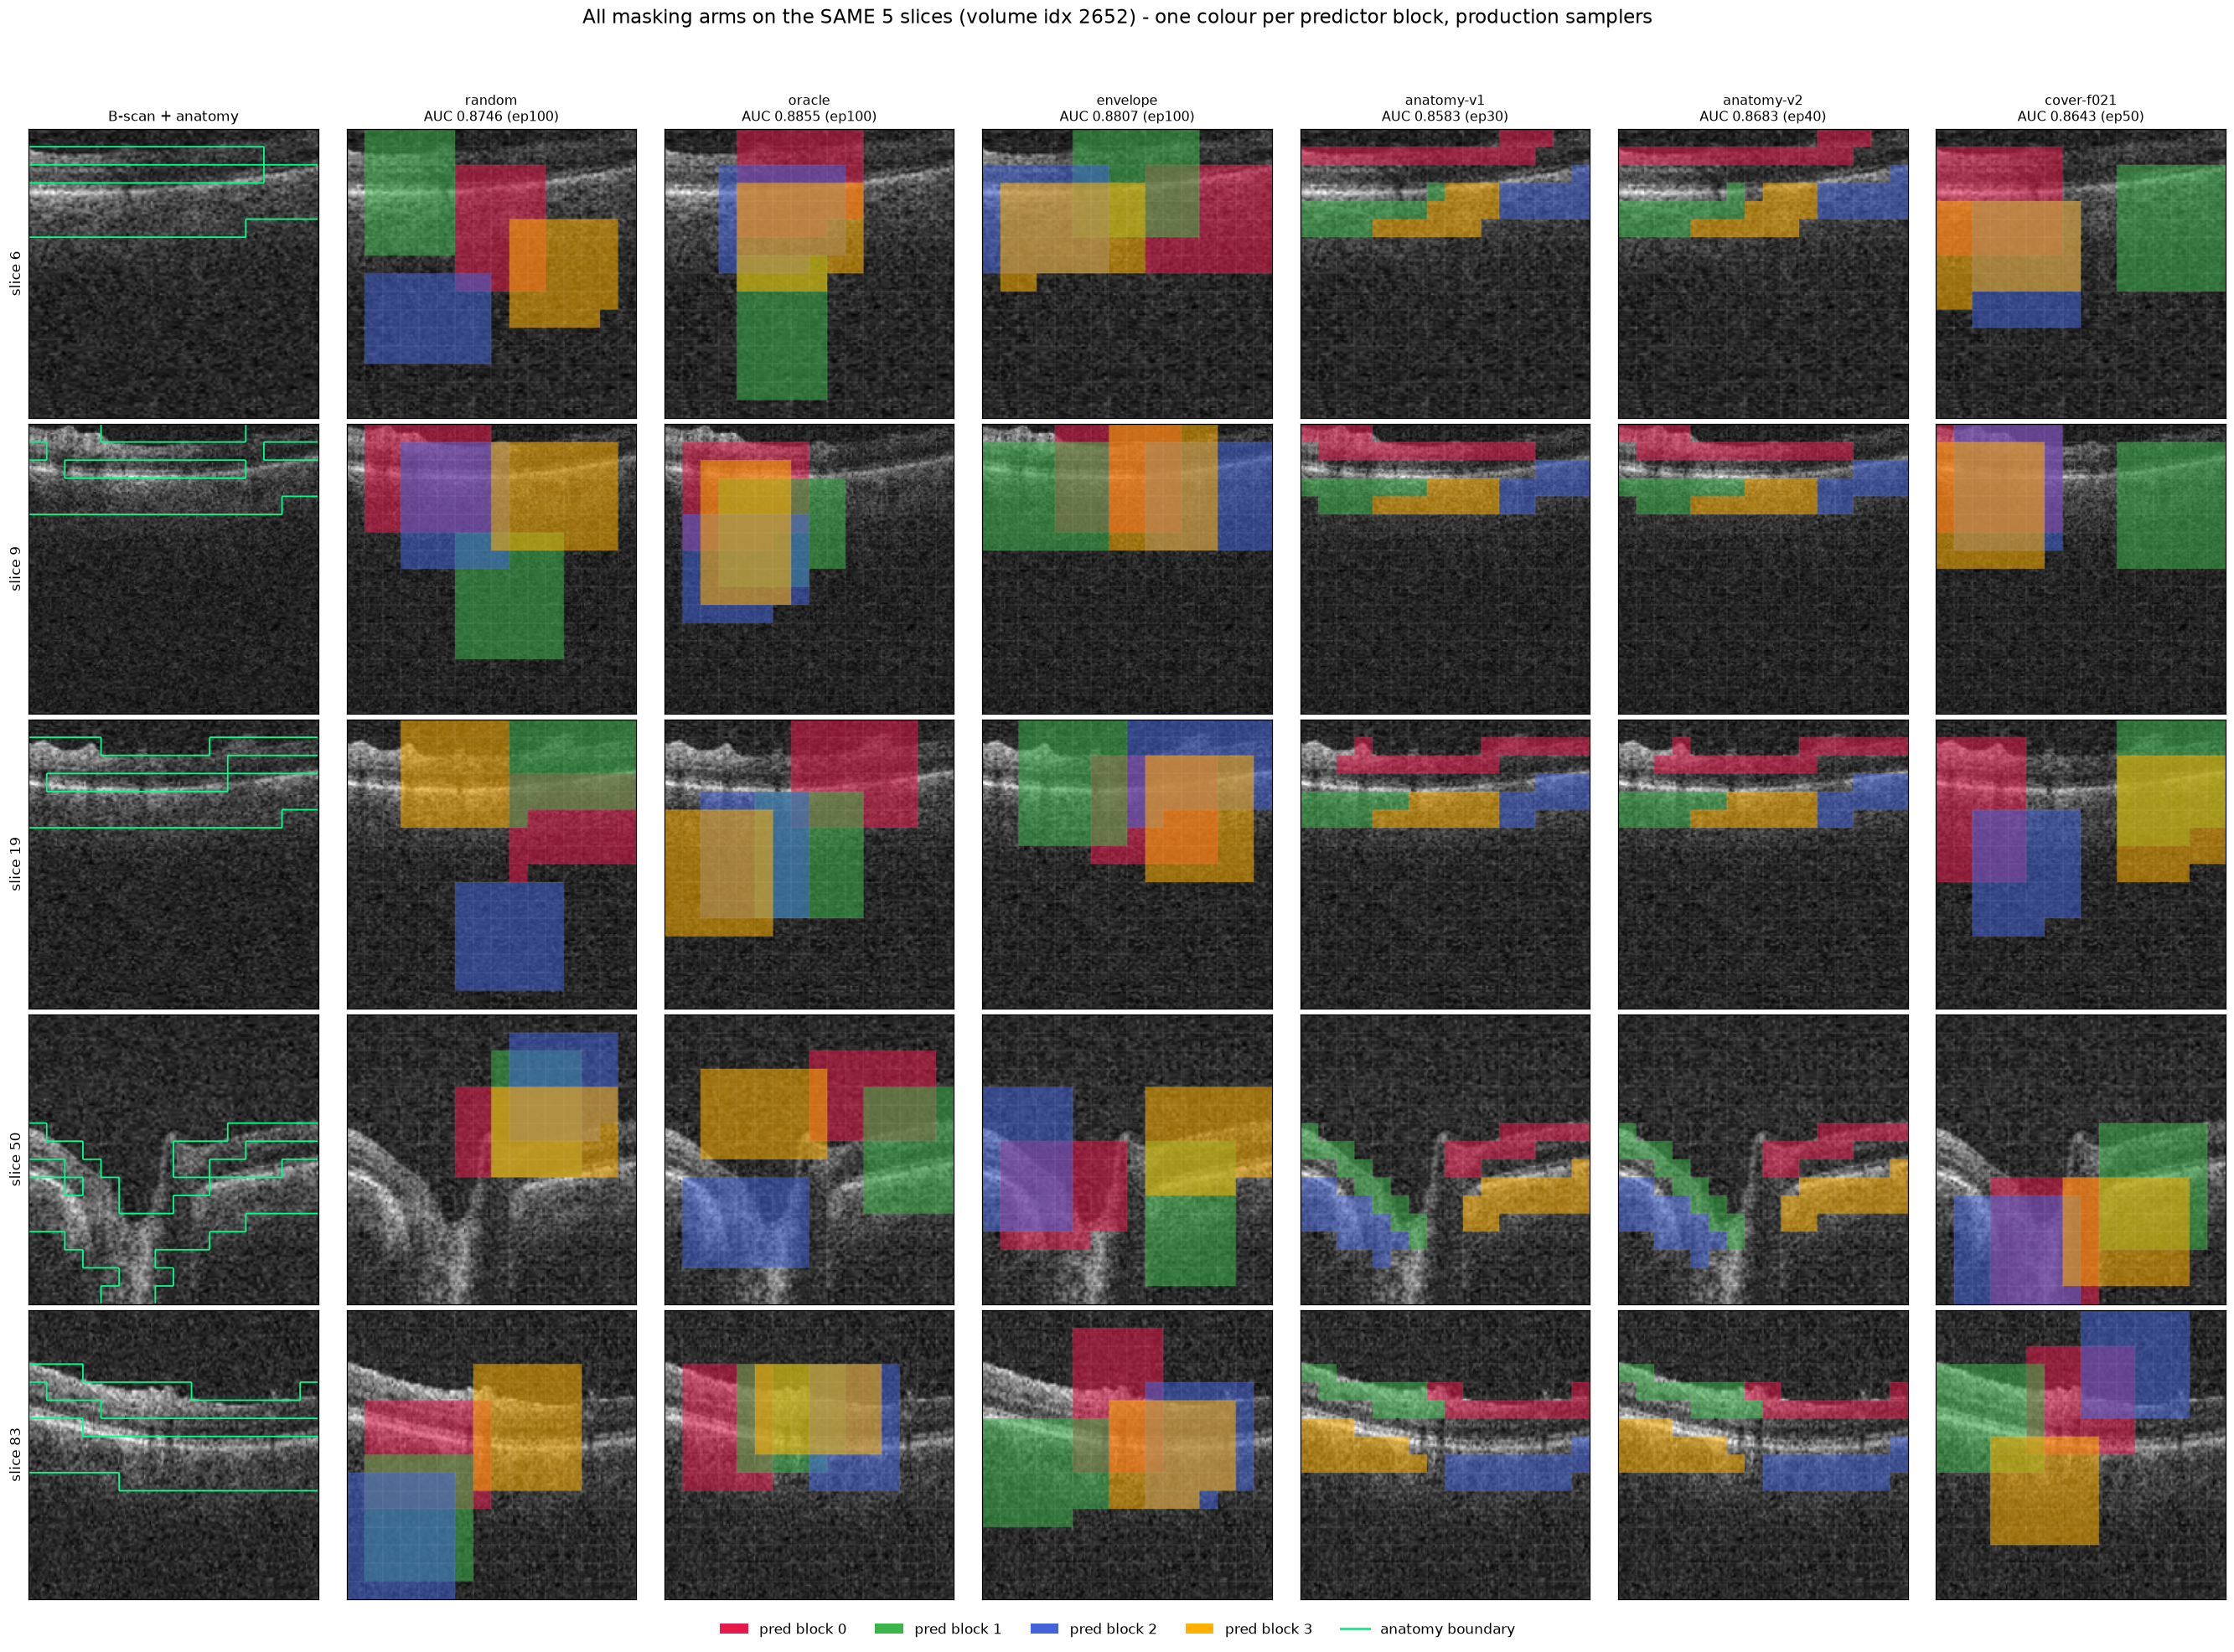
\includegraphics[width=\linewidth]{fig_masking_policies.png}
\caption{The six masking policies on the same five B-scans, drawn with the
production samplers. Each predictor target block has its own colour; the green
contour is the anatomy reference. \textsc{random} places rectangles without
regard to tissue; \textsc{oracle} tracks the retinal band by intensity alone;
\textsc{envelope} and \textsc{cover} place rectangles using a trained segmenter;
the anatomy arms grow ragged targets that follow tissue almost exactly. Masking
precision increases left to right among the guided arms, but downstream AUC does
not (Table~\ref{tab:main}).}
\label{fig:policies}
\end{figure}

\section{Results}

\subsection{Guidance helps; precision does not}

\begin{table}[t]
\centering
\caption{Frozen MeanPool probe, FairVision test ($N{=}3000$). All arms share one
epoch-25 ancestor and one protocol. $\Delta$ is versus \textsc{random} at the
same epoch. Red daggered entries are placeholders for runs in progress.}
\label{tab:main}
\small
\begin{tabular}{llccc}
\toprule
arm & guidance signal & ep50 & ep75 & ep100 \\
\midrule
random           & none (null)                      & 0.8641 & 0.8723 & 0.8746 \\
oracle           & intensity centroid, no segmenter & 0.8740 & 0.8836 & 0.8855 \\
envelope         & trained segmenter                & 0.8761 & 0.8803 & 0.8807 \\
anatomy-v2       & trained segmenter (shape)        & 0.8654 & --     & --     \\
cover $f{=}0.21$ & trained segmenter (coverage)     & 0.8643 & \ph{0.0000} & \ph{0.0000} \\
\midrule
\multicolumn{2}{l}{$\Delta$ cover $-$ random}  & $+0.0002$ & \ph{$+0.0000$} & \ph{$+0.0000$} \\
\multicolumn{2}{l}{$\Delta$ cover $-$ oracle}  & $-0.0097$ & \ph{$+0.0000$} & \ph{$+0.0000$} \\
\bottomrule
\end{tabular}
\end{table}

Table~\ref{tab:main} reports the main comparison. Two results are already firm.
Guidance helps: the \textsc{oracle} band gives $+0.0109$ over the null at epoch
100 (paired bootstrap over test volumes, 95\% CI $[+0.0058,+0.0162]$,
$p<0.0005$), with a stable margin across epochs ($+0.0099$, $+0.0113$,
$+0.0109$). And guidance by a \emph{trained segmenter} is not required to obtain
it: the segmentation-free oracle exceeds the segmenter-guided \textsc{envelope}
arm by $+0.0047$ at epoch 100, while \textsc{envelope}'s own margin over the
null shrinks with training ($+0.0120 \to +0.0080 \to +0.0062$).

The \textsc{cover} arm's epoch-75 and epoch-100 probes are
\phtext{pending; runs in progress} and are required before the coverage
hypothesis can be evaluated. At epoch 50 it is indistinguishable from the null
($+0.0002$).

\subsection{Anatomical precision is not the operative variable}

\begin{table}[t]
\centering
\caption{Measured mask geometry, 600 held-out slices, production samplers.
``purity'' is the fraction of masked cells lying on tissue. All values measured.}
\label{tab:geom}
\small
\begin{tabular}{lccccc}
\toprule
arm & anatomy hidden & purity & mask ratio & context kept & AUC (best ep) \\
\midrule
random           & 52.2\% & 31.6\% & 43.7\% & 42.1\% & 0.8746 \\
oracle           & 62.2\% & 41.1\% & 40.0\% & 45.6\% & 0.8855 \\
envelope         & 76.9\% & 43.5\% & 46.4\% & 40.5\% & 0.8807 \\
cover $f{=}0.21$ & 74.1\% & 45.3\% & 43.3\% & 43.5\% & \ph{0.0000} \\
anatomy-v2       & 80.3\% & \textbf{97.3\%} & 21.4\% & 67.9\% & 0.8654 \\
\bottomrule
\end{tabular}
\end{table}

Table~\ref{tab:geom} measures what each sampler actually does. The result is not
ordered by anatomical targeting: the anatomy arms place $97$--$98\%$ of masked
cells on tissue and rank last, while the oracle places $41\%$ on tissue and
ranks first. Across the four rectangle arms, the Spearman correlation between
fraction-of-anatomy-hidden and AUC is $-0.40$ --- the wrong sign --- and no
measured geometric variable is a significant predictor at this sample size.

The anatomy arms also differ from the rectangle arms on several axes at once:
they leave $68\%$ of tokens as context versus $42\%$, and run at roughly half the
effective masking ratio. We therefore report their deficit but do \textbf{not}
attribute it to target shape; that comparison is confounded by construction.

The \textsc{cover} policy is the intended test of the remaining hypothesis: it
matches the rectangle arms on mask ratio, context, and predictor budget, while
raising anatomy coverage to $74\%$ under an explicit visible-tissue floor. Its
outcome is \phtext{pending}.

\subsection{Subgroup analysis}

Joining saved test predictions to demographics in deterministic loader order
(validated by exact label reconstruction), Black participants have the lowest
AUC in every valid probe. The disparity persists across masking policies and
epochs, suggesting it is inherited from the data and downstream task rather than
introduced by the pretraining objective.

\subsection{Reproducibility}

The epoch-100 oracle encoder and its trained probe head are public. Re-encoding
the test split on different hardware, at fp32 rather than fp16, and with a
different encoder chunk size reproduces the reported AUC to $9.8\times10^{-6}$
($0.8854754$ versus $0.8854852$): 22 discordant pairs out of $2{,}248{,}844$.
Probe-time numerical precision is therefore immaterial to every comparison here.

\section{Limitations}

\textbf{One pretraining run per policy.} The paired bootstrap quantifies
sampling error on a fixed test set, not seed-to-seed variance of pretraining.
With $n{=}1$ continuation per arm the \emph{ranking} is not established even
where individual pairwise differences are significant. This is the principal
limitation.

\textbf{One visible-tissue floor.} Only $f{=}0.21$ is pretrained, so we report
no dose-response over the floor and make no claim that any floor is optimal.

\textbf{Confounded shape comparison.} The anatomy arms differ in masking ratio,
context size, and number of predictor loss terms simultaneously; we do not use
them to support a causal claim about target shape.

\textbf{Single dataset and task.} Glaucoma classification on FairVision OCT only.

\section{Conclusion}

Guidance of masked-prediction targets helps on retinal OCT, but a trained
segmentation model is not required to obtain it, and increasing the anatomical
precision of the mask is associated with worse rather than better
representations. Whether an explicit visible-tissue floor recovers the benefit of
anatomy coverage is the open question this study is designed to answer, and its
resolution is \phtext{pending completion of the $f{=}0.21$ run}.

\bibliographystyle{plainnat}
\bibliography{references}

\end{document}
